\documentclass[a4paper]{article}
\usepackage{graphicx}
\usepackage{onecolceurws}

\title{KAT: an Annotation Tool for STEM Documents}

\author{
Felix Schmoll
\and
Tom Wiesing
\and
Michael Kohlhase
}

\institution{Jacobs University Bremen}




\begin{document}
\maketitle

\begin{abstract}

\end{abstract}
\vskip 32pt


\section{Introduction}

\subsection{Document Annotation Tools}

\subsection{Modalities of STEM documents}

\subsection {Requirements for Linguistic Annotations for Structured Documents}

\section{Editing Annotations in the browser}
%explain from ground up, not say how it was before

There are three different modes that can be chosen via buttons in the sidebar. They each represent a different mode of working with the annotations.


%what are the design decisions, and why where were they made (why is more important than the what)
\subsection{Creating Annotations}
In its essence an annotation is a selection of text that is enriched with additional information. KAT implements in that a text section can be chosen and via a right-click event different annotation categories from the KAnnSpec can be chosen. A form opens up in a sidebar where the information can be entered. This is natural as KAT is a browser-based tool, where forms are the standard way of entering information. It is also the easiest way to ensure formalization.

\begin{figure}[htbp]
 \centering
 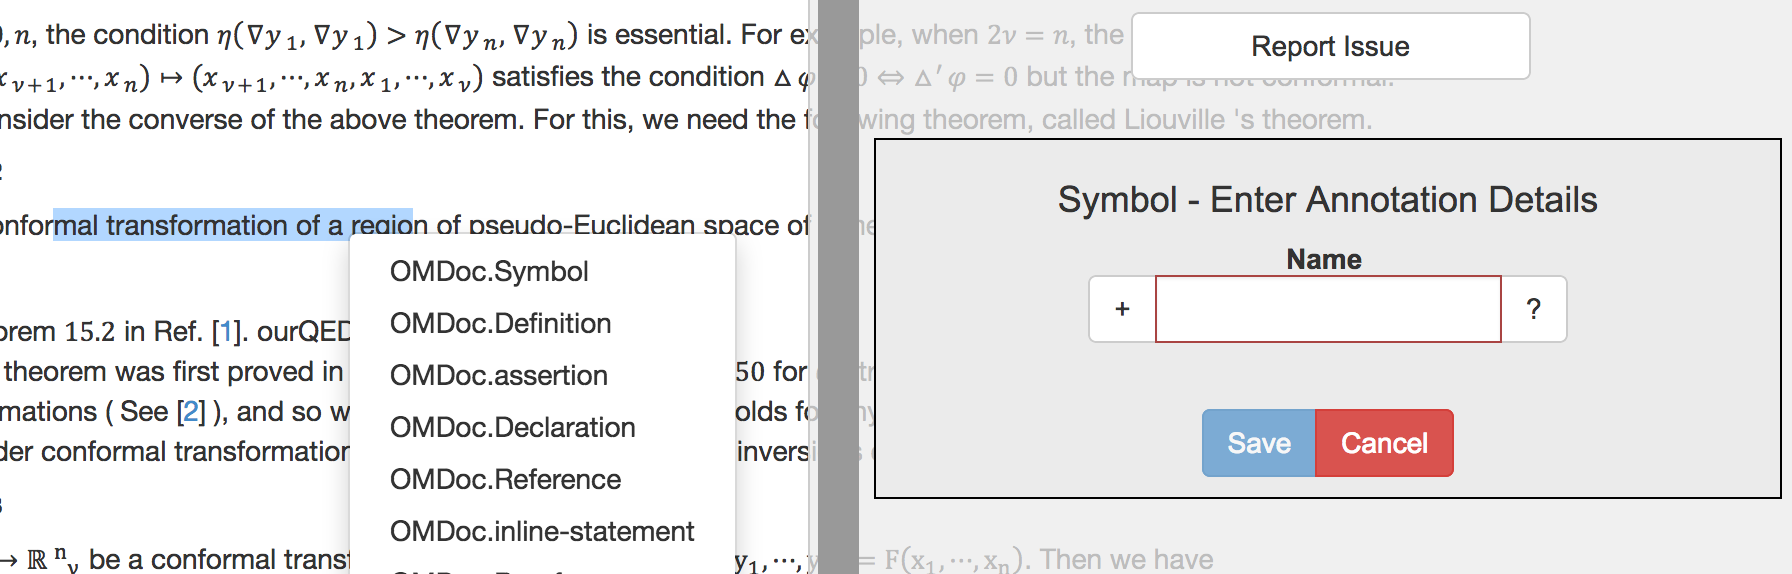
\includegraphics[width=0.8\textwidth]{annotation_creation.png}
 \caption{Creating annotation in KAT.}
\end{figure}

\subsection{Review mode}
After annotations have been created it is possible to evaluate them using a special review mode. The idea is that here automatically created (e.g. with [Frederik's thesis]) annotations can be evaluated by a human operator. The annotations can be iterated through by going forward and backwards in the order of appearance in the document. For each annotation then one can endorse it or flag it.

\subsection{Visualizing Annotations}


%references
%2-3 pages
%sunday lunch time

\section{Future Work \& Conclusion}

	\begin{enumerate}
		\item \emph{Distinction between annotations.} - Currently we distinguish different annotation categories by color and give them a transparent opacity s.t. one can see if multiple annotations overlap. The color mapping is however not injective and it becomes difficult once there are more than two annotations overlapping.
	\end{enumerate}
	
	%reference to Frederik's work

\subsubsection{Acknowledgements}





%\bibliographystyle{alpha} 
%\bibliography{samplebib}
%inline the .bbl file directly for mailing to authors.

\begin{thebibliography}{Com79}

\bibitem[Gin15]{KAT-paper}
Deyan Ginev, Sourabh Lal, Michael Kohlhase and Tom Wiesing.
\newblock KAT: an Annotation Tool for STEM Documents.
\newblock {\em CERMAT}, September 2015.


\end{thebibliography}

\end{document}


